Gli strumenti utilizzati per questo esperimento sono stati:
\begin{itemize}
    \item Il \textbf{pendolo di Maxwell} (Fig. \ref{pendolo_di_maxwel}), composto da quattro oggetti fondamentali: un piedistallo, un'impalcatura, due fili e il disco di cui misurare il momento d'inerzia.
    \item Il \textbf{disco non omogeneo} di plastica (Fig. \ref{disco}), composto da quattro toroidi concentrici con al centro il perno metallico appeso ai fili del il pendolo di Maxwell.
     \begin{figure}[htbp]
        \centering
        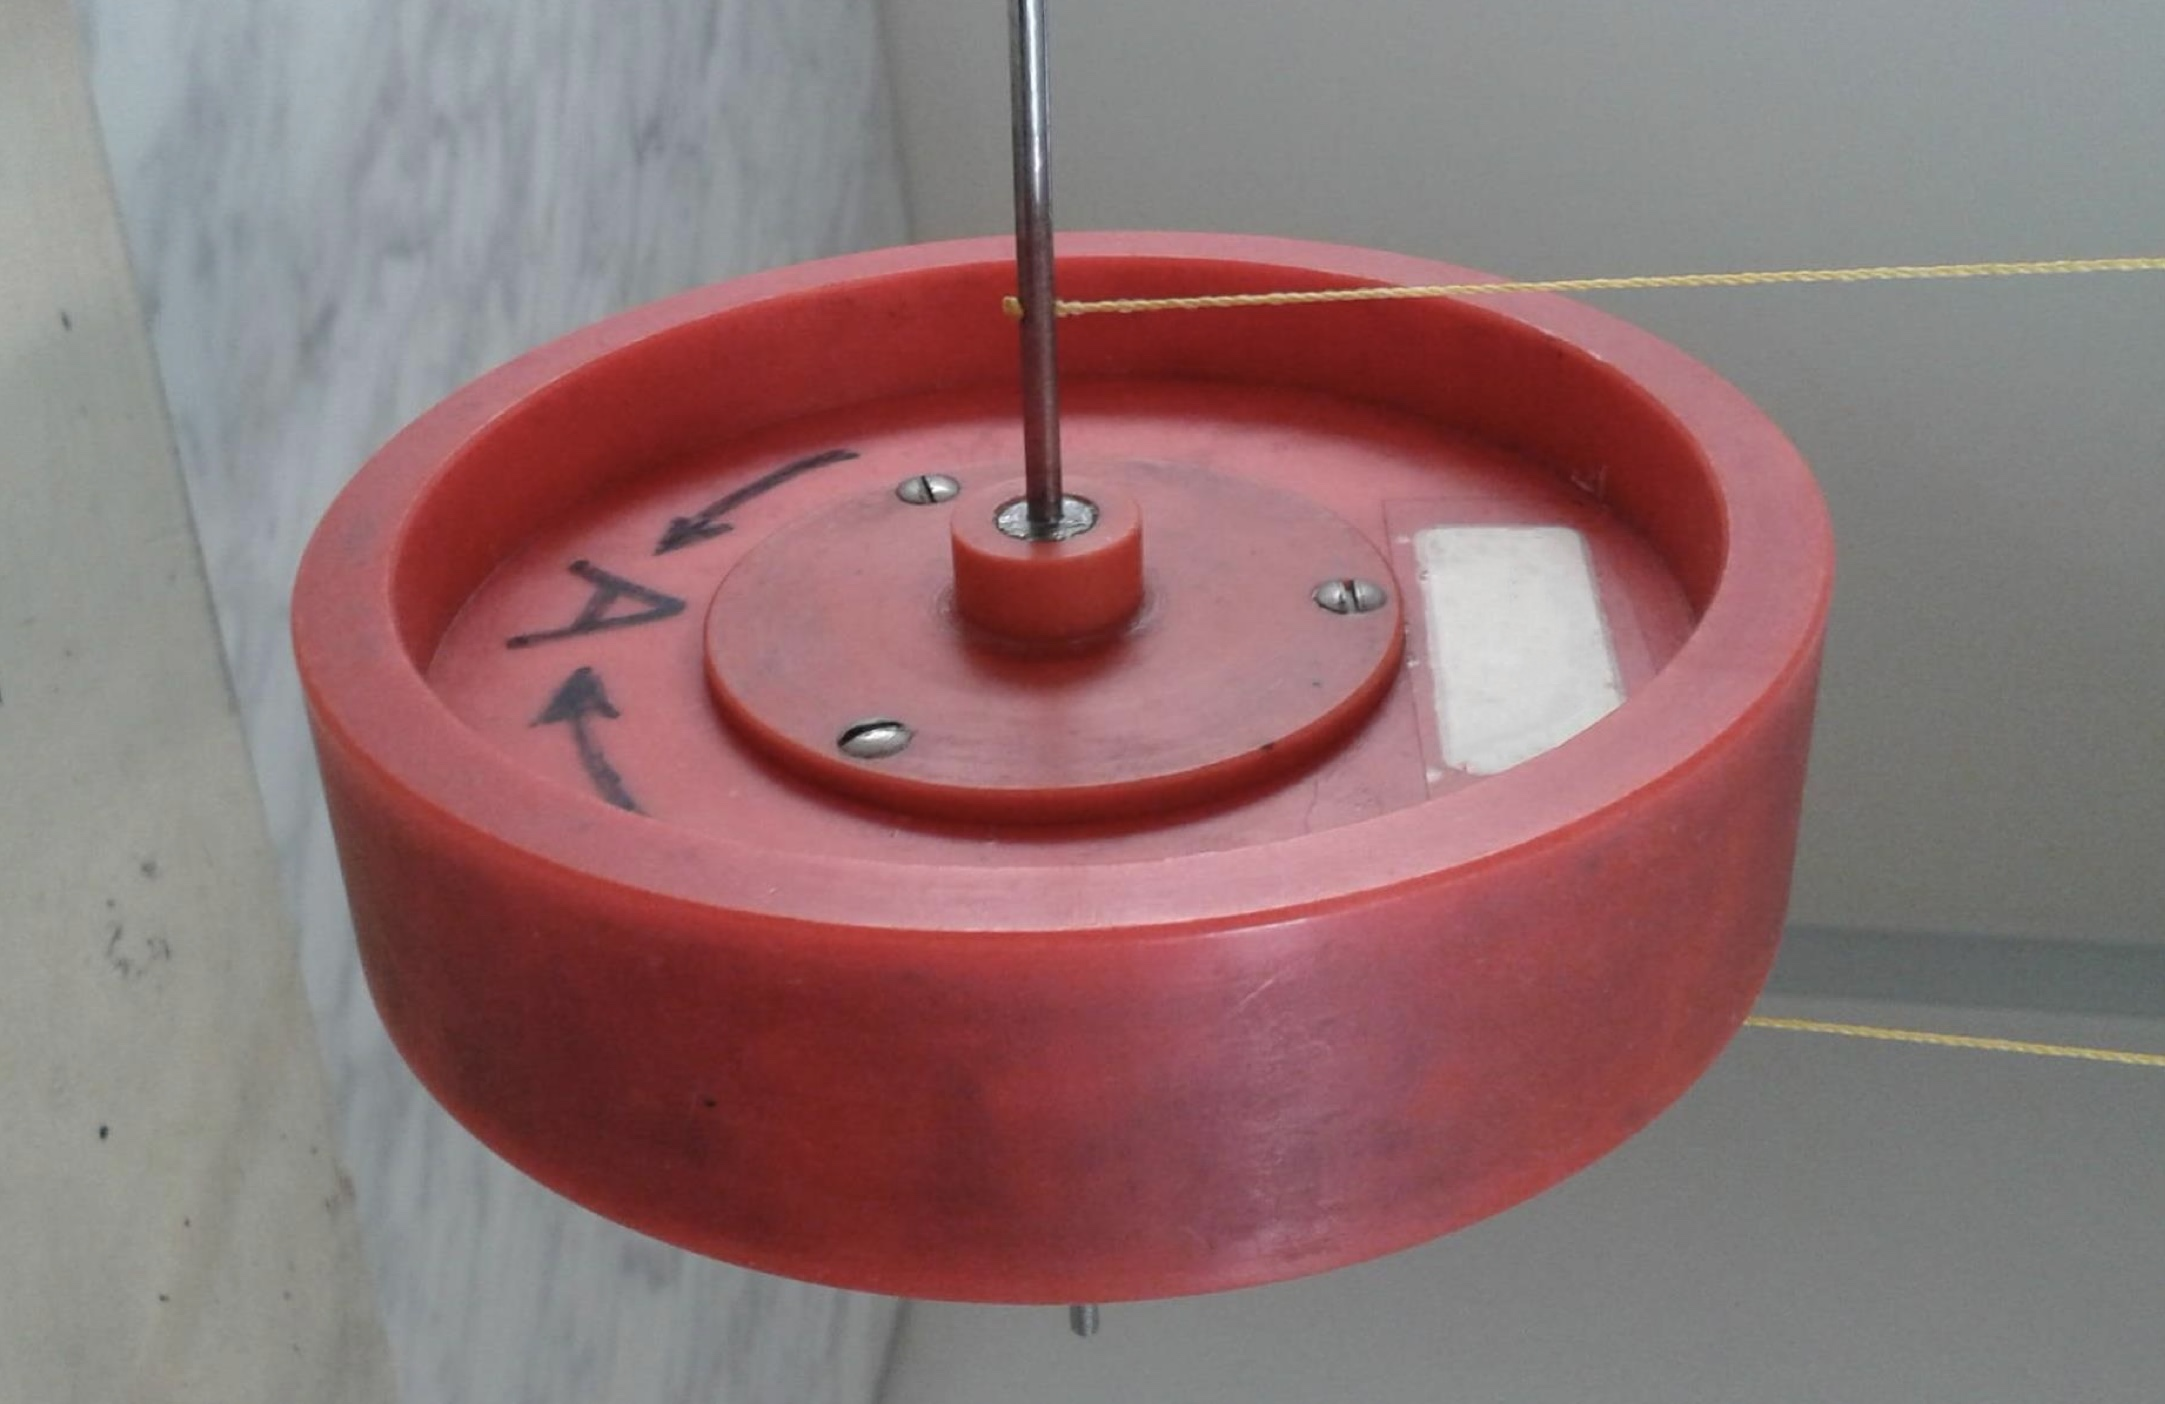
\includegraphics[width=0.70\textwidth]{image/Disco.jpeg}
        \caption[\small Il disco non omogeneo.]{\small Il disco non omogeneo di cui calcolare il momento d'inerzia è composta da quattro toroidi concentrici. Al centro di esso vi è il perno metallico appeso ai due fili del pendolo di Maxwell}
        \label{disco}
    \end{figure}\\
    \item Un \textbf{cronometro digitale} (risoluzione: 0.01 s) di uno smartphone.
    \item Un \textbf{calibro digitale} (risoluzione: 0.01 mm) munito di ganasce da muovere manualmente.
    \item Un \textbf{micrometro manuale} (risoluzione: 0.01 mm) munito di ganasce che vengono mosse da una vite micrometrica, fatta girare manualmente da un tamburo.
    \item Un \textbf{metro a nastro} metallico (risoluzione: 1 mm).
    \begin{figure}[htbp]
        \centering
        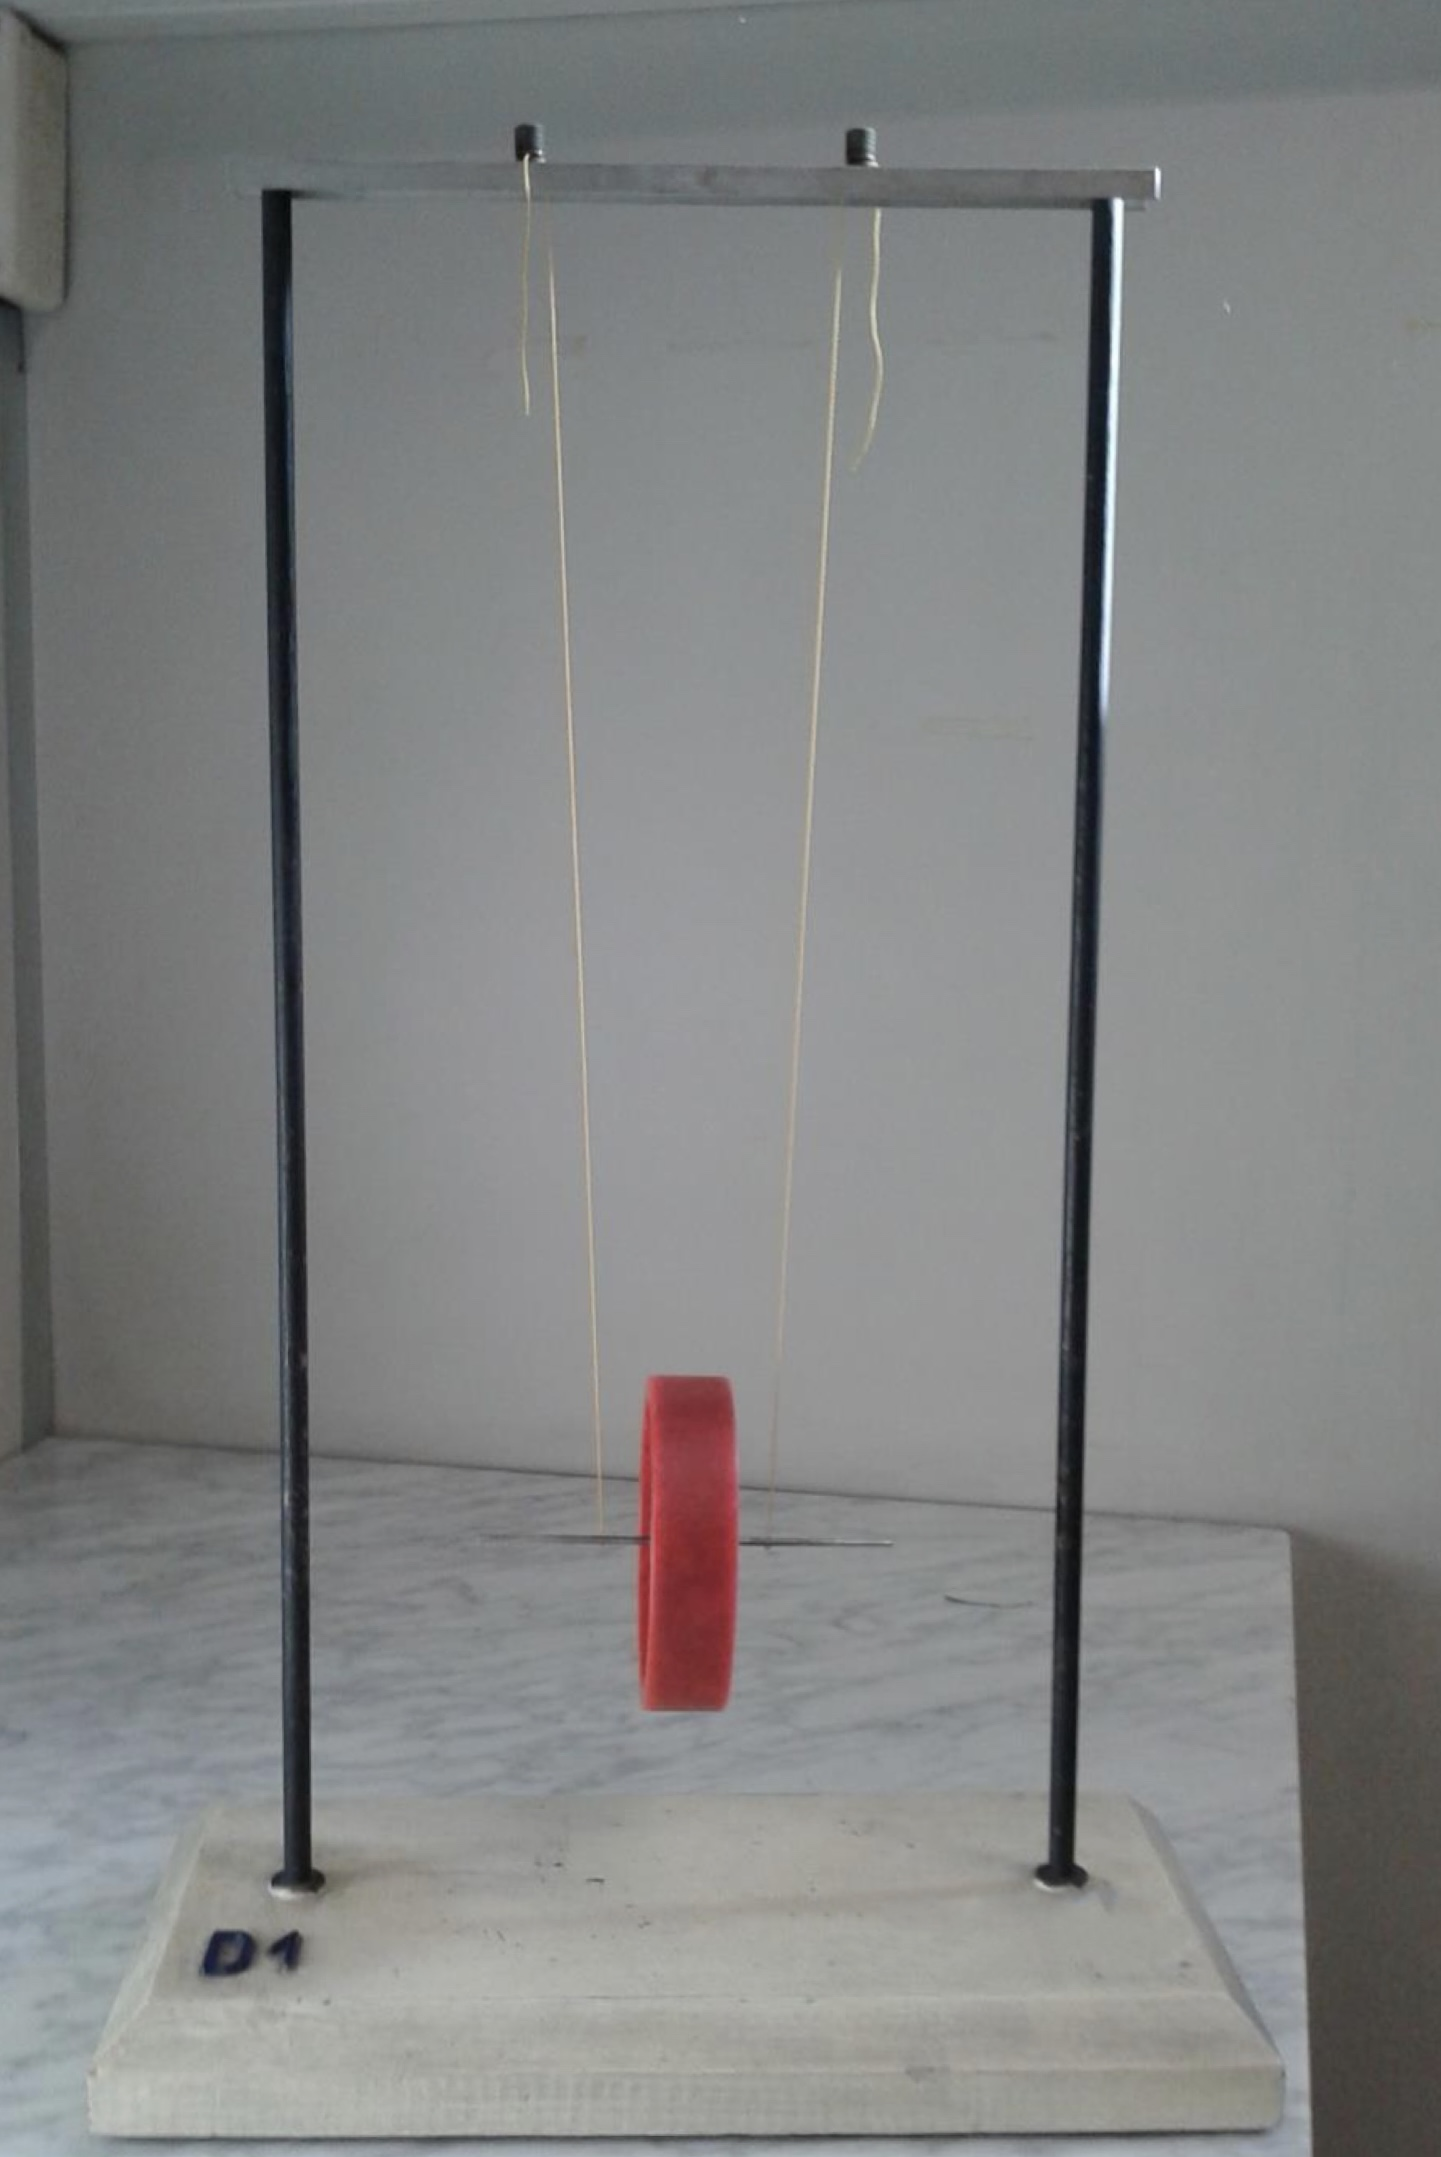
\includegraphics[width=0.65\textwidth]{image/Pendolo_di_Maxwell.jpeg}
        \caption[\small Il pendolo di Maxwell.]{\small Il pendolo di Maxwell con vista frontale: il disco di cui misurare il momento d'inerzia è appeso ai fili che sono fissati all'impalcatura dell'apparato.}
        \label{pendolo_di_maxwel}
    \end{figure}\\
\end{itemize}